\subsection{End-to-End Evaluation}
\todo{We take the best featurization from the previous section and apply it to the following datasets}

% ALL OF JIGSAWS RESULTS
\begin{figure*}[!ht]
	\centering
	\begin{subfigure}[t]{7in}
	    \centering
        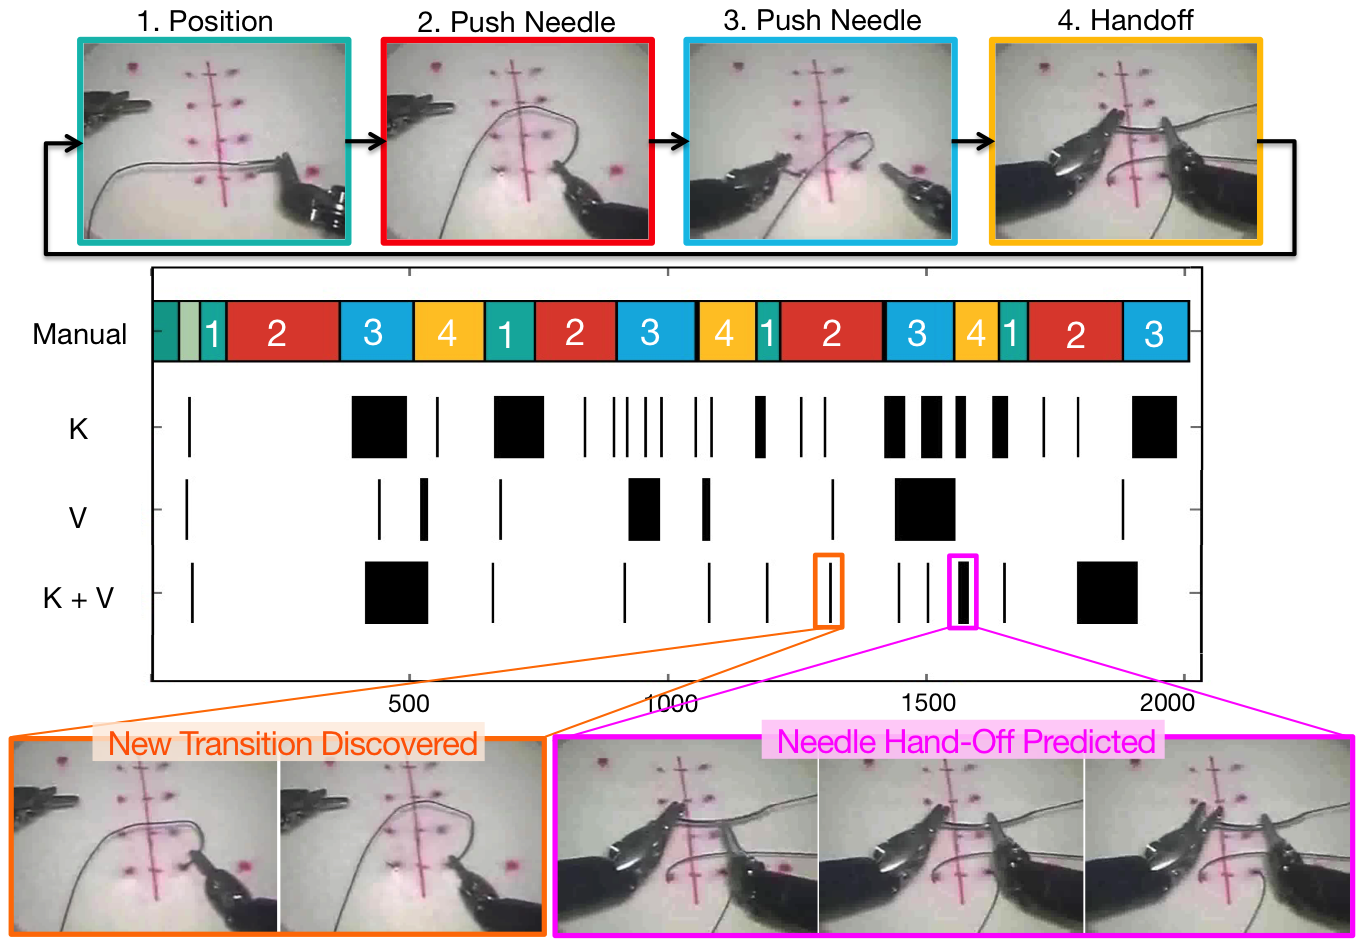
\includegraphics[width=0.8\linewidth]{figures/suturing}
		\caption{Suturing}
		\label{fig:suturing}
% 		\vspace{-5pt}
	\end{subfigure}
	\begin{subfigure}[t]{0.5\textwidth}
	    \vspace{0pt}
	    \centering
		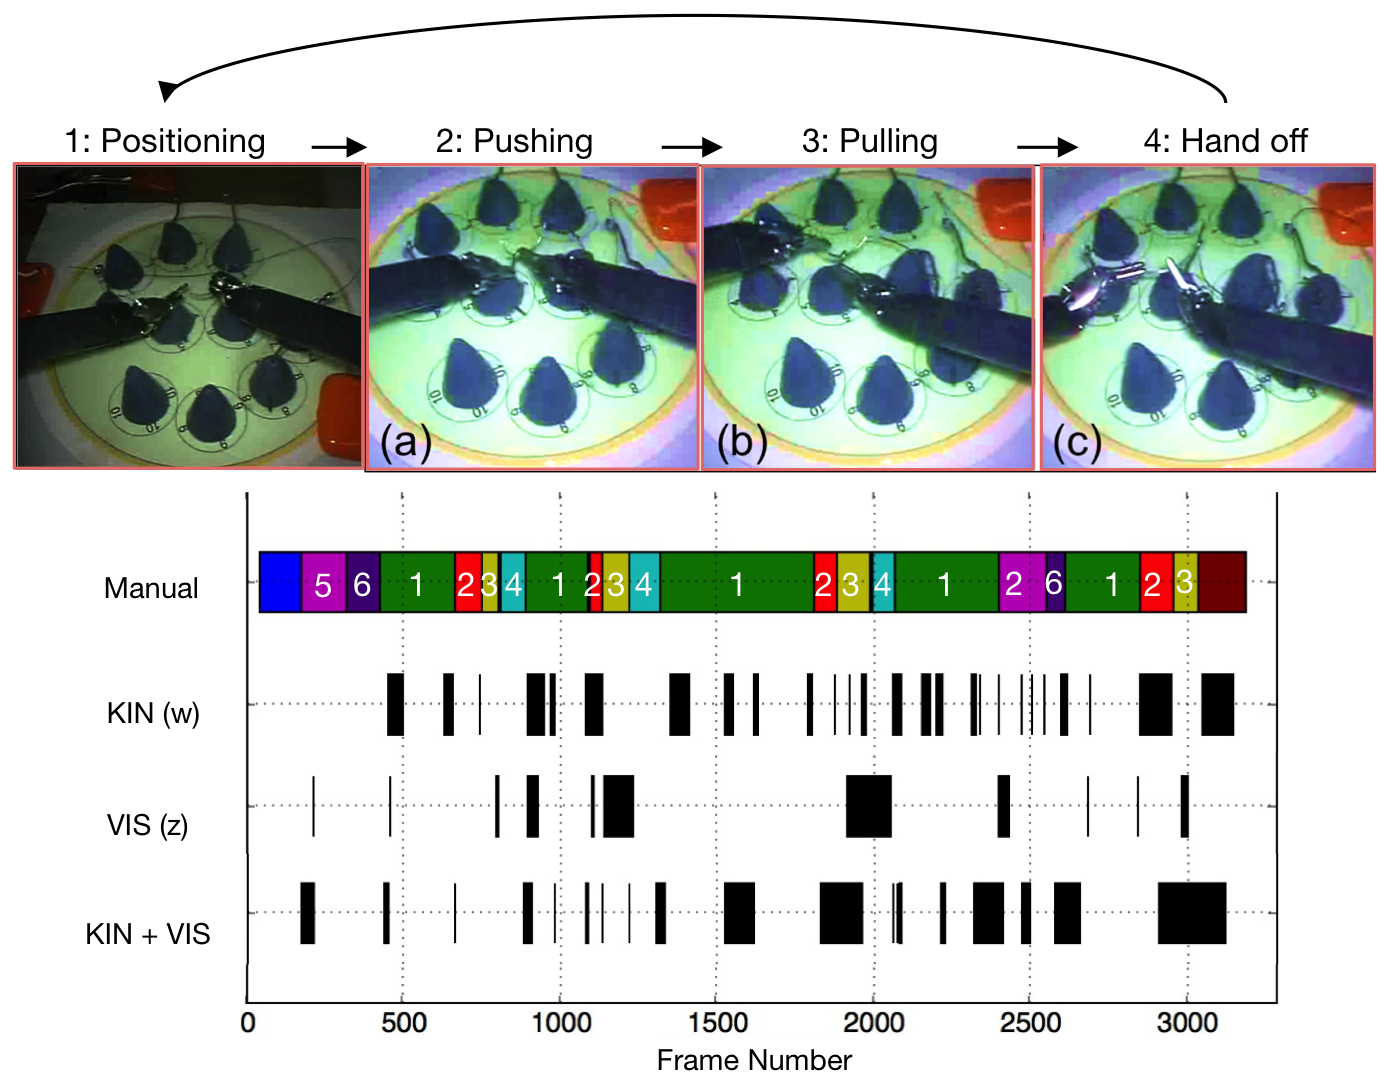
\includegraphics[width=\linewidth]{figures/needle_passing}
		\caption{Needle Passing}
		\label{fig:needlePassing}
		\par\vspace{0pt}
	\end{subfigure}
	\quad
	\begin{subfigure}[t]{0.4\textwidth}
            \vspace{0pt}
            \centering
            \resizebox{\linewidth}{!}{% put in textwidth
                \begin{tabular}{ll|l|l|l|l|l|l}
                \multicolumn{2}{c}{}                                     &     \multicolumn{3}{c}{\cellcolor[HTML]{CBCEFB}Silhouette Score} & \multicolumn{3}{c}{\cellcolor[HTML]{FFC72C}DTW Score}\\
                \multicolumn{2}{c}{}    & \multicolumn{1}{c|}{K} & \multicolumn{1}{c|}{Z} & \multicolumn{1}{c|}{K+Z}& \multicolumn{1}{c|}{K} & \multicolumn{1}{c|}{Z} & \multicolumn{1}{c}{K+Z} \\ \hline \hline 
                \rowcolor[HTML]{E0E0E0}
                \cellcolor[HTML]{CBCEFB}                                 & E     & &    &   &   &  &    \\ 
                \cellcolor[HTML]{CBCEFB}                                 & E+I   & &    &   &   &  &    \\ 
                \rowcolor[HTML]{E0E0E0}
                \multirow{-3}{*}{\cellcolor[HTML]{CBCEFB}Suturing}       & E+I+N & &    &   &   &  &    \\ 
                \cellcolor[HTML]{FFC72C}                                 & E     & &    &   &   &  &    \\ 
                \rowcolor[HTML]{E0E0E0}
                \cellcolor[HTML]{FFC72C}                                 & E+I   & &    &   &   &  &    \\ 
                \multirow{-3}{*}{\cellcolor[HTML]{FFC72C}\parbox{1.2cm}{Needle Passing}} & E+I+N & &    &   &   &  &    \\ \hline
                \end{tabular}
            }
            \caption{TABLE III: Comparison of \TSC performance on Suturing and Needle Passing Tasks. We compare the prediction performance by incrementally adding demonstrations from Experts~(E), Intermediates~(I), and Novices~(N) respectively to the dataset.\todo{Experiments running on machine, also handle whitespece}}
            \label{tab:jigsaws}
            \par\vspace{0pt}
	\end{subfigure}
	\caption{\todo{fix figure} The figure shows a sequence of images for the Suturing and Needle Passing tasks in JIGSAWS dataset\cite{gao2014jigsaws}.
The first row shows a manual segmentation of the task in 4 semantic steps: (1) Needle Positioning, (2) Needle Pushing, (3) Pulling Needle, (4) Hand-off.
Both these tasks require 4 repetitions of the full 4 step cycle and run for approx. 100s (frame numbers are at 30 fps).
We show the sub-task level segmentation results from our completely unsupervised approach with only Kinematics data, only Visual data and a concatenation of both tasks with multiple spurious segments as in \figref{needlePassing} and \ref{fig:suturing}. \figref{suturing} also shows (in magenta) frames of predicted Needle Hand-off, and (in orange) a new transition for needle re-orientation between needle push and needle pull.
}
	\label{fig:jigsaws}
	\vspace{-15pt}
\end{figure*}


% \subsubsection{Synthetic Example}
\vspace{5pt}
\noindent \textbf{1. Synthetic Example: }
A Synthetic example with a robot in blue and target in yellow is shown in \figref{toyEx}. The robot moves to the target, and a new target appears after the robot has reached the current target. Each demonstration episode consists of 4 targets, where the target $i$ is sampled from  $\sim\,\mathcal{N}(\mu_i, 1)$ where $\mu_i$ is randomly generated in the first episode and maintained constant across subsequent episodes. For these examples, we generate 5 episodes of each individual setting.

\figref{toyEx} (b) shows the results of unsupervised segmentation into the 4 steps -- each time the robot reaches the target-- using only kinematics data ($\binom{x(t)}{y(t)}$). The results for this preliminary example align the transitions with changes in directions robots motions affirming our correctness of model for hierarchical clustering. 

We further evaluate the effect of partial observability, by reducing the state dimension to only $(x(t))$. As expected, the our method only has a component of the gradient, and hence the uncertainty on the output transitions increases, albeit around the correct mean. 

Next, we introduce control noise in the system, $x(t+1) = x(t)+u(t)+\nu$, where $\nu\, \sim\, \mathcal{N}(0, d_1)$ where varying $d_1\in[0,1]$. The \figref{toyEx} (c) shows the results for $d_1=0.25$. Similar to the previous experiment we experiment with full kinematics along with partial observability. We find that in case of noise, one dimensional trajectory can have drifts which would erroneously show up as transitions. 
We also evaluate the performance of segmentation using only Visual features, specifically SIFT features. We observe that the segments are correctly identified, however due to the nature of SIFT feautures, transitions have longer time lengths.
Finally, we note that a combination of Kinematics and Visual features allows disambiguation from noise, and hence allows for sharper transition clusters than either of those independently. 

Next, we introduce a kinematic sensor noise in the system $\hat{x}(t)= x(t)+\nu$, where $\nu\, \sim\, \mathcal{N}(0, d_2)$ where varying $d_2\in[0,1]$. The \figref{toyEx} (c) shows the results for $d_2=0.25$. We note that only the kinematics is corrupted with noise, while the vision sees a perfectly straight trajectory. We first segment using full kinematic state. Thereafter we use partially observed state as in the aforementioned case. We observe that in this case, the segmentation performance substantially degrades. Then, we use SIFT visual features as in previous experiment. We find improved transitions based only on videos. We then combine with partially observed state, this results in slight improvement, and combination with full kinematics state with noise yields drastic improvements in segmentaiton performance. 

%===============================================================
%PR2 figures
\begin{figure*}[ht!]
	\centering
	\begin{subfigure}[t]{3.4in}
	    \centering
        
\includegraphics[width=0.5\linewidth]{figures/insert}
		\caption{The figure illustrates the performance of unsupervised segmentation of the 3 Step Lego Assembly Task performed with tele-operated PR2 with two techniques of manual demonstrations.}
		\figlabel{lego-pr2}
		\vspace{-5pt}
	\end{subfigure}
	 \hspace{0.1in}
	\begin{subfigure}[t]{3.4in}
	    \centering
		
\includegraphics[width=0.5\linewidth]{figures/insert}
		\caption{The figure illustrates the comparison of unsupervised segmentation of the Toy Example performed with tele-operated PR2 with two techniques of manual demonstrations.}
		\figlabel{toyPlane-pr2human}
		\vspace{-5pt}
	\end{subfigure}
	\caption{\todo{fix figure: Similar figure as for JIGSAWS dataset}}
	\figlabel{pr2_expts}
	\vspace{-15pt}
\end{figure*}

% \begin{figure}[!t]
% \centering
% 
\includegraphics[width=\linewidth]{figures/insert.png}
% \caption{The figure illustrates the performance of unsupervised segmentation of the 3 Step Lego Assembly Task performed with tele-operated PR2 with two techniques of manual demonstrations.}
%  \label{fig:lego-pr2}
% \vspace{-10pt} 
% \end{figure}

% \begin{figure}[!t]
% \centering
% 
\includegraphics[width=\linewidth]{figures/insert.png}
% \caption{The figure illustrates the comparison of unsupervised segmentation of the Toy Example performed with tele-operated PR2 with two techniques of manual demonstrations.}
%  \label{fig:toyPlane-pr2human}
% \vspace{-10pt} 
% \end{figure}

% \subsubsection{PR2: Legos and Toy Plane Assembly}
\vspace{5pt}
\noindent \textbf{2. PR2: Legos and Toy Plane Assembly: }
This experiment involves a multi-step assembly task using (1) large \textit{Lego} blocks and (2) toy \textit{Plane} from the YCB dataset~\cite{calli2015corr}. The data is collected through kinesthetic demonstrations of the task on the PR2 in various situations by the user. 

The \textit{Lego} assembly tasks involves (a) putting red block on top of green, and (b) then putting blue block on top of red. The base green block is fixed while the other two are randomly initialized. The \textit{Plane} assembly task starts with a fixed part placement. The steps in the task are: grasp fuselage, transfer fuselage on the lower wing, grasp top wing, transfer wing on top of fuselage. It is worth noting that parts in both these tasks have interlocking components which require alignment for fitting. Hence intermediate orientations are important before proceeding in the task. 

We collect 8 kinesthetic demonstrations for each task and use \TSC for learning unsupervised segmentation. the results of one example each of the \textit{Lego} and \textit{Plane} assembly task is illustrated in Figures~\ref{fig:lego-pr2} and \ref{fig:pr2_toyplane} respectively.

% \subsubsection{Human Demonstration of Toy Plane Assembly}
\vspace{5pt}
\noindent \textbf{3. Human Demonstration of Toy Plane Assembly: }
We extend the experiment of the toy plane assembly to collect 8 demonstrations each from two separate human users. We note that in these cases, we only record video and have no kinematic information. 8 demonstrations from each user are collected, and we note that there was a difference between users in the grasping location of fuselage. We used \TSC to learn segmentation for human demonstrations and the results are showed in \figref{toyPlane-pr2human}.

The results for clustering evaluation and comparison with a set of manual labels using dynamic time warping distance are tabulated in \tabref{pr2}.

\begin{table}[t!]
\centering
\caption{Comparison of \TSC performance on Plane and Lego Assembly Tasks \todo{Experiments running on machine}}
\label{tab:pr2}
\begin{tabular}{l|l|l|l|l|l|l}
\multicolumn{1}{c}{}                                     &     \multicolumn{3}{c}{\cellcolor[HTML]{CBCEFB}Silhouette Score} & \multicolumn{3}{c}{\cellcolor[HTML]{FFC72C}DTW Score}\\
\multicolumn{1}{c}{}    & \multicolumn{1}{c|}{K} & \multicolumn{1}{c|}{Z} & \multicolumn{1}{c|}{K+Z}& \multicolumn{1}{c|}{K} & \multicolumn{1}{c|}{Z} & \multicolumn{1}{c}{K+Z} \\ \hline \hline 
\rowcolor[HTML]{E0E0E0}
 Lego (Robot)    & &    &   &   &  &    \\ 
 Plane (Robot)   & &    &   &   &  &    \\ 
\rowcolor[HTML]{E0E0E0}
 Plane (Person 1) & &    &   &   &  &    \\ 
 Plane (Person 2)      & &    &   &   &  &    \\  \hline
\end{tabular}
\vspace{-10pt}
\end{table}


%===============================================================

% \subsubsection{Surgical Subtask Segmentation}
\vspace{5pt}
\noindent \textbf{4. Surgical Subtask Segmentation: }
We apply our method to the JIGSAWS dataset\cite{gao2014jigsaws} consisting of surgical task demonstrations under tele-operation using the da~Vinci surgical system. The dataset was captured from eight surgeons with different levels of skill, performing five repetitions each of suturing and needle passing.

\vspace{0.5em}
\noindent\textit{Suturing: }We have explored 39 examples of a 4 throw suturing task (\figref{suturing}). Using the right arm, the first step is to penetrate one of the points on right side. The next step is to force the needle through the phantom to the other side. Using the left arm, the robot pulls the needle out of the phantom, and then hands it off to the right arm for the next point. Qualitative results from the suturing task are illustrated in \figref{suturing}.
\todo{Discuss: Recovery of transitions which have manual labels, and discovery of new transitions.}

\vspace{0.5em}
\noindent\textit{Needle Passing: } Next, we applied our framework to 28 demonstrations of the needle passing task.
The robot passes a needle through a loop using its right arm, then its left arm to pull the needle through the loop. Then, the robot hands the needle off from the left arm to the right arm. This is repeated four times, as illustrated with a manual segmentation in \figref{needlePassing}. It also shows the predicted segmentation for the same trajectory example. 

\tabref{jigsaws} lists results for unsupervised evaluation and similarity with a set of manual labels. We show results for increasingly complex datasets: Experts only (E), E+ Intermediates (E+I), and E+I+Novices(E+I+N). We compare results from kinematics, visual and combined set of features.


\iffalse
\subsubsection{Evaluation of Results }

\noindent \textit{Exp1. End-to-end result with some task}

\begin{enumerate}
\item Show that clusters are sensible and align with some intuitive criteria e.g., surgemes
\end{enumerate}

\noindent \textit{Exp2. Does Vision Help}

\begin{enumerate}
\item Remove visual features and show that clusters degrade
\end{enumerate}

\noindent \textit{Exp3. Parameter Search}

\begin{enumerate}
\item Describe our eval procedure and how we arrived at the architecture we did.
\end{enumerate}

\noindent \textit{Robustness}
\begin{enumerate}
\item Add noise or corrupt images and test to see how robust the segmentations we learn are.
\end{enumerate}
\fi

\iffalse
\subsection{Discussion}
\begin{enumerate}
\item How successful was our unsupervised approach in learning meaningful segmentations
\item RGB videos vs. RGB-D videos
\end{enumerate}
\fi